\documentclass{standalone}
\usepackage{tikz}
\usetikzlibrary{patterns, positioning}


\begin{document}
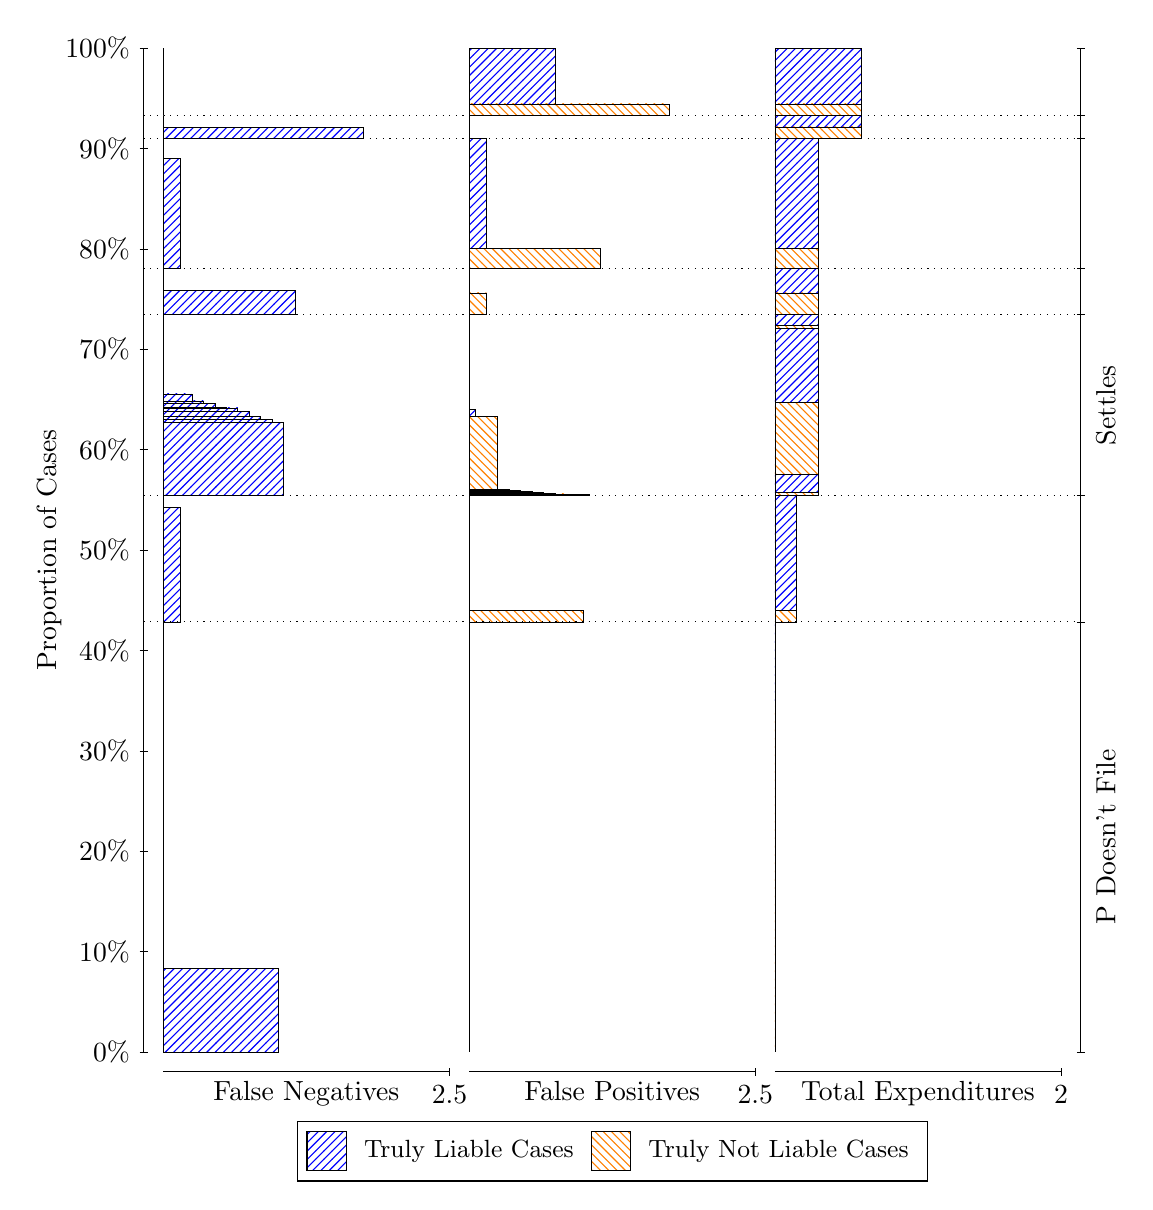
\begin{tikzpicture}
\draw[black, very thin] (1.5,1.75) -- (1.5,14.5);
\node[rotate=90, text=black, anchor=center] at (0.3, 8.125) {Proportion of Cases};
\draw[black, very thin] (1.45,1.75) -- (1.55,1.75);
\node[text=black, anchor=east] at (1.45, 1.75) {0\%};
\draw[black, very thin] (1.45,3.025) -- (1.55,3.025);
\node[text=black, anchor=east] at (1.45, 3.025) {10\%};
\draw[black, very thin] (1.45,4.3) -- (1.55,4.3);
\node[text=black, anchor=east] at (1.45, 4.3) {20\%};
\draw[black, very thin] (1.45,5.575) -- (1.55,5.575);
\node[text=black, anchor=east] at (1.45, 5.575) {30\%};
\draw[black, very thin] (1.45,6.85) -- (1.55,6.85);
\node[text=black, anchor=east] at (1.45, 6.85) {40\%};
\draw[black, very thin] (1.45,8.125) -- (1.55,8.125);
\node[text=black, anchor=east] at (1.45, 8.125) {50\%};
\draw[black, very thin] (1.45,9.4) -- (1.55,9.4);
\node[text=black, anchor=east] at (1.45, 9.4) {60\%};
\draw[black, very thin] (1.45,10.675) -- (1.55,10.675);
\node[text=black, anchor=east] at (1.45, 10.675) {70\%};
\draw[black, very thin] (1.45,11.95) -- (1.55,11.95);
\node[text=black, anchor=east] at (1.45, 11.95) {80\%};
\draw[black, very thin] (1.45,13.225) -- (1.55,13.225);
\node[text=black, anchor=east] at (1.45, 13.225) {90\%};
\draw[black, very thin] (1.45,14.5) -- (1.55,14.5);
\node[text=black, anchor=east] at (1.45, 14.5) {100\%};

\draw[black, very thin] (13.4,1.75) -- (13.4,14.5);
\draw[black, very thin] (13.35,1.75) -- (13.45,1.75);
\node[anchor=west] at (13.35, 1.75) {};
\draw[black, very thin] (13.35,7.2119) -- (13.45,7.2119);
\node[anchor=west] at (13.35, 7.2119) {};
\draw[black, very thin] (13.35,8.8148) -- (13.45,8.8148);
\node[anchor=west] at (13.35, 8.8148) {};
\draw[black, very thin] (13.35,11.113) -- (13.45,11.113);
\node[anchor=west] at (13.35, 11.113) {};
\draw[black, very thin] (13.35,11.703) -- (13.45,11.703);
\node[anchor=west] at (13.35, 11.703) {};
\draw[black, very thin] (13.35,13.349) -- (13.45,13.349);
\node[anchor=west] at (13.35, 13.349) {};
\draw[black, very thin] (13.35,13.643) -- (13.45,13.643);
\node[anchor=west] at (13.35, 13.643) {};
\draw[black, very thin] (13.35,14.5) -- (13.45,14.5);
\node[anchor=west] at (13.35, 14.5) {};

\draw[black, very thin, pattern color=blue, pattern=north east lines] (1.75,1.75) rectangle (3.2033,2.8152);
\draw[black, very thin, pattern color=orange, pattern=north west lines] (1.75,2.8152) rectangle (1.75,7.2119);
\draw[black, very thin, pattern color=blue, pattern=north east lines] (1.75,7.2119) rectangle (1.968,8.6676);
\draw[black, very thin, pattern color=orange, pattern=north west lines] (1.75,8.6676) rectangle (1.75,8.8148);
\draw[black, very thin, pattern color=blue, pattern=north east lines] (1.75,8.8148) rectangle (3.276,9.7483);
\draw[black, very thin, pattern color=blue, pattern=north east lines] (1.75,9.7483) rectangle (3.1307,9.7842);
\draw[black, very thin, pattern color=blue, pattern=north east lines] (1.75,9.7842) rectangle (2.9853,9.823);
\draw[black, very thin, pattern color=blue, pattern=north east lines] (1.75,9.823) rectangle (2.84,9.8847);
\draw[black, very thin, pattern color=blue, pattern=north east lines] (1.75,9.8847) rectangle (2.6947,9.9293);
\draw[black, very thin, pattern color=blue, pattern=north east lines] (1.75,9.9293) rectangle (2.5493,9.9379);
\draw[black, very thin, pattern color=blue, pattern=north east lines] (1.75,9.9379) rectangle (2.404,9.9894);
\draw[black, very thin, pattern color=blue, pattern=north east lines] (1.75,9.9894) rectangle (2.2587,10.018);
\draw[black, very thin, pattern color=blue, pattern=north east lines] (1.75,10.018) rectangle (2.1133,10.109);
\draw[black, very thin, pattern color=orange, pattern=north west lines] (1.75,10.109) rectangle (1.75,11.113);
\draw[black, very thin, pattern color=blue, pattern=north east lines] (1.75,11.113) rectangle (3.4213,11.425);
\draw[black, very thin, pattern color=orange, pattern=north west lines] (1.75,11.425) rectangle (1.75,11.703);
\draw[black, very thin, pattern color=blue, pattern=north east lines] (1.75,11.703) rectangle (1.968,13.096);
\draw[black, very thin, pattern color=orange, pattern=north west lines] (1.75,13.096) rectangle (1.75,13.349);
\draw[black, very thin, pattern color=blue, pattern=north east lines] (1.75,13.349) rectangle (4.2933,13.493);
\draw[black, very thin, pattern color=orange, pattern=north west lines] (1.75,13.493) rectangle (1.75,13.643);
\draw[black, very thin, pattern color=orange, pattern=north west lines] (1.75,13.643) rectangle (1.75,13.79);
\draw[black, very thin, pattern color=blue, pattern=north east lines] (1.75,13.79) rectangle (1.75,14.5);
\draw[black, very thin, pattern color=orange, pattern=north west lines] (5.6333,1.75) rectangle (5.6333,6.1467);
\draw[black, very thin, pattern color=blue, pattern=north east lines] (5.6333,6.1467) rectangle (5.6333,7.2119);
\draw[black, very thin, pattern color=orange, pattern=north west lines] (5.6333,7.2119) rectangle (7.0867,7.359);
\draw[black, very thin, pattern color=blue, pattern=north east lines] (5.6333,7.359) rectangle (5.6333,8.8148);
\draw[black, very thin, pattern color=orange, pattern=north west lines] (5.6333,8.8148) rectangle (7.1593,8.8268);
\draw[black, very thin, pattern color=orange, pattern=north west lines] (5.6333,8.8268) rectangle (7.014,8.8309);
\draw[black, very thin, pattern color=orange, pattern=north west lines] (5.6333,8.8309) rectangle (6.8687,8.8383);
\draw[black, very thin, pattern color=orange, pattern=north west lines] (5.6333,8.8383) rectangle (6.7233,8.8405);
\draw[black, very thin, pattern color=orange, pattern=north west lines] (5.6333,8.8405) rectangle (6.578,8.8548);
\draw[black, very thin, pattern color=orange, pattern=north west lines] (5.6333,8.8548) rectangle (6.4327,8.8554);
\draw[black, very thin, pattern color=orange, pattern=north west lines] (5.6333,8.8554) rectangle (6.4327,8.8727);
\draw[black, very thin, pattern color=orange, pattern=north west lines] (5.6333,8.8727) rectangle (6.2873,8.8852);
\draw[black, very thin, pattern color=orange, pattern=north west lines] (5.6333,8.8852) rectangle (6.142,8.8969);
\draw[black, very thin, pattern color=orange, pattern=north west lines] (5.6333,8.8969) rectangle (5.9967,9.8186);
\draw[black, very thin, pattern color=blue, pattern=north east lines] (5.6333,9.8186) rectangle (5.706,9.9101);
\draw[black, very thin, pattern color=blue, pattern=north east lines] (5.6333,9.9101) rectangle (5.6333,11.113);
\draw[black, very thin, pattern color=orange, pattern=north west lines] (5.6333,11.113) rectangle (5.8513,11.391);
\draw[black, very thin, pattern color=blue, pattern=north east lines] (5.6333,11.391) rectangle (5.6333,11.703);
\draw[black, very thin, pattern color=orange, pattern=north west lines] (5.6333,11.703) rectangle (7.3047,11.956);
\draw[black, very thin, pattern color=blue, pattern=north east lines] (5.6333,11.956) rectangle (5.8513,13.349);
\draw[black, very thin, pattern color=orange, pattern=north west lines] (5.6333,13.349) rectangle (5.6333,13.499);
\draw[black, very thin, pattern color=blue, pattern=north east lines] (5.6333,13.499) rectangle (5.6333,13.643);
\draw[black, very thin, pattern color=orange, pattern=north west lines] (5.6333,13.643) rectangle (8.1767,13.79);
\draw[black, very thin, pattern color=blue, pattern=north east lines] (5.6333,13.79) rectangle (6.7233,14.5);
\draw[black, very thin, pattern color=orange, pattern=north west lines] (9.5167,1.75) rectangle (9.5167,6.1467);
\draw[black, very thin, pattern color=blue, pattern=north east lines] (9.5167,6.1467) rectangle (9.5167,7.2119);
\draw[black, very thin, pattern color=orange, pattern=north west lines] (9.5167,7.2119) rectangle (9.7892,7.359);
\draw[black, very thin, pattern color=blue, pattern=north east lines] (9.5167,7.359) rectangle (9.7892,8.8148);
\draw[black, very thin, pattern color=orange, pattern=north west lines] (9.5167,8.8148) rectangle (10.062,8.8554);
\draw[black, very thin, pattern color=blue, pattern=north east lines] (9.5167,8.8554) rectangle (10.062,9.0824);
\draw[black, very thin, pattern color=orange, pattern=north west lines] (9.5167,9.0824) rectangle (10.062,10.004);
\draw[black, very thin, pattern color=blue, pattern=north east lines] (9.5167,10.004) rectangle (10.062,10.938);
\draw[black, very thin, pattern color=orange, pattern=north west lines] (9.5167,10.938) rectangle (10.062,10.979);
\draw[black, very thin, pattern color=blue, pattern=north east lines] (9.5167,10.979) rectangle (10.062,11.113);
\draw[black, very thin, pattern color=orange, pattern=north west lines] (9.5167,11.113) rectangle (10.062,11.391);
\draw[black, very thin, pattern color=blue, pattern=north east lines] (9.5167,11.391) rectangle (10.062,11.703);
\draw[black, very thin, pattern color=orange, pattern=north west lines] (9.5167,11.703) rectangle (10.062,11.956);
\draw[black, very thin, pattern color=blue, pattern=north east lines] (9.5167,11.956) rectangle (10.062,13.349);
\draw[black, very thin, pattern color=orange, pattern=north west lines] (9.5167,13.349) rectangle (10.607,13.499);
\draw[black, very thin, pattern color=blue, pattern=north east lines] (9.5167,13.499) rectangle (10.607,13.643);
\draw[black, very thin, pattern color=orange, pattern=north west lines] (9.5167,13.643) rectangle (10.607,13.79);
\draw[black, very thin, pattern color=blue, pattern=north east lines] (9.5167,13.79) rectangle (10.607,14.5);
\draw[black, dotted] (1.5,7.2119) -- (13.4,7.2119);
\draw[black, dotted] (1.5,8.8148) -- (13.4,8.8148);
\draw[black, dotted] (1.5,11.113) -- (13.4,11.113);
\draw[black, dotted] (1.5,11.703) -- (13.4,11.703);
\draw[black, dotted] (1.5,13.349) -- (13.4,13.349);
\draw[black, dotted] (1.5,13.643) -- (13.4,13.643);
\draw[black, very thin] (1.75,1.5) -- (5.3833,1.5);
\node[text=black, anchor=north] at (3.5667, 1.5) {False Negatives};
\draw[black, very thin] (5.3833,1.45) -- (5.3833,1.55);
\node[text=black, anchor=north] at (5.3833, 1.45) {2.5};

\draw[black, very thin] (5.6333,1.5) -- (9.2667,1.5);
\node[text=black, anchor=north] at (7.45, 1.5) {False Positives};
\draw[black, very thin] (9.2667,1.45) -- (9.2667,1.55);
\node[text=black, anchor=north] at (9.2667, 1.45) {2.5};

\draw[black, very thin] (9.5167,1.5) -- (13.15,1.5);
\node[text=black, anchor=north] at (11.333, 1.5) {Total Expenditures};
\draw[black, very thin] (13.15,1.45) -- (13.15,1.55);
\node[text=black, anchor=north] at (13.15, 1.45) {2};

\node[text=black, centered, rotate=90] at (13.72, 4.4809) {P Doesn't File};

\node[text=black, centered, rotate=90] at (13.72, 9.964) {Settles};





\draw (7.449999999999999,1.5) node[draw=none] (baseCoordinate) {};
\begin{scope}[align=center]
        \matrix[scale=0.5, draw=black, below=0.5cm of baseCoordinate, nodes={draw}, column sep=0.1cm]{
            \node[rectangle, draw, minimum width=0.5cm, minimum height=0.5cm, pattern color=blue, pattern=north east lines] {}; &
            \node[draw=none, font=\small, text=black] (B) {Truly Liable Cases}; &
            \node[rectangle, draw, minimum width=0.5cm, minimum height=0.5cm, pattern color=orange, pattern=north west lines] {}; &
            \node[draw=none, font=\small, text=black] (B) {Truly Not Liable Cases}; \\
            };
\end{scope}

\end{tikzpicture}
\end{document}